\section{SQuAD Item Examples}
\label{ch:isicle:apx:examples}

Figures~\ref{fig:ex-disc-neg}, \ref{fig:ex-feas}, \ref{fig:ex-reasonable}, and \ref{fig:ex-tricky} show previously discussed \squad{} examples (\S\ref{ch:isicle:interp}) in full.
The \squad{} annotations from Figure~\ref{fig:example-error} are included in supplementary materials and at \projecturl{}.
On the same page, we provide a web interface for inspecting the parameters of the \irt{} models.
Figure~\ref{fig:lambda-dist} shows the feasibility distribution corresponding to Figure~\ref{fig:irt-dist}.


\begin{figure*}[t]
  \center
  \small
  \tikz\node[draw=black!40!lightblue,inner sep=1pt,line width=0.3mm,rounded corners=0.1cm]{
    \begin{tabular}{p{.95\textwidth}}
      \textbf{\Discability{}}: -9.63 \textbf{\Diff{}}: -0.479 \textbf{Feasibility}: 0.614 \textbf{Mean Exact Match}: 0.472 \\
      \textbf{Wikipedia Page}: \underline{Economic inequality}  \textbf{Question ID:} 572a1c943f37b319004786e3             \\
      \textbf{Question}: Why did the demand for rentals decrease?                                                          \\
      \textbf{Official Answer}: \answer{demand for higher quality housing}                                                 \\
      \textbf{Context}:
      A number of researchers (David Rodda, Jacob Vigdor, and Janna Matlack), argue that a shortage of affordable housing – at least in the US – is caused in part by income inequality. David Rodda noted that from 1984 and 1991, the number of quality rental units decreased as the \answer{demand for higher quality housing increased} (Rhoda 1994:148). Through gentrification of older neighbourhoods, for example, in East New York, rental prices increased rapidly as landlords found new residents willing to pay higher market rate for housing and left lower income families without rental units. The ad valorem property tax policy combined with rising prices made it difficult or impossible for low income residents to keep pace.
    \end{tabular}
  };

  \caption{
    The example from \squad{} with the lowest \discability{}. Surprisingly, it had a \textit{negative} \discability{}, implying that the less skilled a \subj{} is, the more likely their response is to be correct.
  }
  \label{fig:ex-disc-neg}
\end{figure*}

\begin{figure*}[t]
  \center
  \small
  \tikz\node[draw=black!40!lightblue,inner sep=1pt,line width=0.3mm,rounded corners=0.1cm]{
    \begin{tabular}{p{.95\textwidth}}
      \textbf{\Discability{}}: 3.24 \textbf{\Diff{}}: 3.86 \textbf{Feasibility}: 0 \textbf{Mean Exact Match}: 0            \\
      \textbf{Wikipedia Page}: \underline{Computational Complexity Theory}  \textbf{Question ID:} 56e1b00ce3433e14004230a1 \\
      \textbf{Question}: In the determination of complexity classes, what are two examples of types of Turing machines?    \\
      \textbf{Official Answer}: \answer{probabilistic Turing machines, non-deterministic Turing machines}                  \\
      \textbf{Context}:
      Many types of Turing machines are used to define complexity classes, such as deterministic Turing machines, probabilistic Turing machines, non-deterministic Turing machines, quantum Turing machines, symmetric Turing machines and alternating Turing machines. They are all equally powerful in principle, but when resources (such as time or space) are bounded, some of these may be more powerful than others.
    \end{tabular}
  };

  \caption{
    This question is regarded as infeasible by the \irt{} model.
    Upon further inspection, the answer omits five acceptable answers, but more importantly does not permit all combinations of Turing machines.
  }
  \label{fig:ex-feas}
\end{figure*}

\begin{figure*}[t]
  \center
  \small
  \tikz\node[draw=black!40!lightblue,inner sep=1pt,line width=0.3mm,rounded corners=0.1cm]{
    \begin{tabular}{p{.95\textwidth}}
      \textbf{\Discability{}}: 2.1 \textbf{\Diff{}}: 2.38 \textbf{Feasibility}: 0.995 \textbf{Mean Exact Match}: 0.00621 \textbf{Mean F1}:  0.546 \\
      \textbf{Wikipedia Page}: \underline{European Union Law}  \textbf{Question ID:} 57268f2bf1498d1400e8e3c4
      \\
      \textbf{Question}: What reform was attempted following the Nice Treaty?                                                                     \\
      \textbf{Official Answer}: \answer{an attempt to reform the constitutional law of the European Union and make it more transparent}           \\
      \textbf{Context}:
      Following the Nice Treaty, there was an attempt to reform the constitutional law of the European Union and make it more transparent; this would have also produced a single constitutional document. However, as a result of the referendum in France and the referendum in the Netherlands, the 2004 Treaty establishing a Constitution for Europe never came into force. Instead, the Lisbon Treaty was enacted. Its substance was very similar to the proposed constitutional treaty, but it was formally an amending treaty, and – though it significantly altered the existing treaties – it did not completely replace them.
    \end{tabular}
  };

  \caption{
    This example shows that the answer span is likely too large, causing models to fail in both \squad{}'s exact match and F1 metrics.
  }
  \label{fig:ex-reasonable}
\end{figure*}

\begin{figure*}[t]
  \center
  \small
  \tikz\node[draw=black!40!lightblue,inner sep=1pt,line width=0.3mm,rounded corners=0.1cm]{
    \begin{tabular}{p{.95\textwidth}}
      \textbf{\Discability{}}: 8.01 \textbf{\Diff{}}: -1.41 \textbf{Feasibility}: 0.939 \textbf{Mean Exact Match}: 0.64 \textbf{Mean F1}:  0.667 \\
      \textbf{Wikipedia Page}: \underline{Normas}  \textbf{Question ID:} 56de10b44396321400ee2595
      \\
      \textbf{Question}: Who did the Normans team up with in Anatolia?                                                                           \\
      \textbf{Official Answer}: \answer{Turkish forces}                                                                                          \\
      \textbf{Context}:
      Some Normans joined Turkish forces to aid in the destruction of the Armenians vassal-states of Sassoun and Taron in far eastern Anatolia. Later, many took up service with the Armenian state further south in Cilicia and the Taurus Mountains. A Norman named Oursel led a force of "Franks" into the upper Euphrates valley in northern Syria.\ldots
    \end{tabular}
  };

  \caption{
    This highly discriminative question succeeds because there are many plausible answers.
    For example, although only ``Turkish forces'' is correct, some models answer ``the Armenian state.''
  }
  \label{fig:ex-tricky}
\end{figure*}


\begin{figure}[t]
  \centering
  \small
  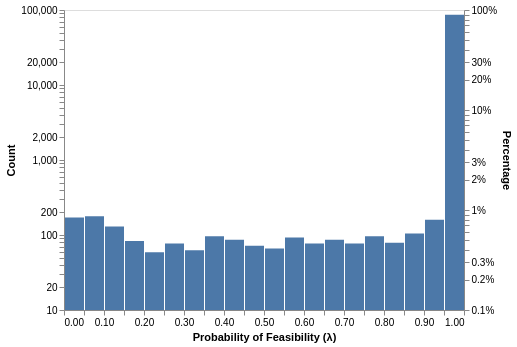
\includegraphics[width=\columnwidth]{irt_lambda_dist}
  \caption{
    The feasibility parameter $\lambda$ of our \irt{} model represents the probability that an example is unsolvable.
    For example, annotation error could lead to an example always being scored incorrectly---regardless of how good the model is.
    In \squad{} 2.0, $\lambda<.434$ in the $5\%$ percentile, $\lambda<.698$ for the $7.5\%$, and $\lambda<.931$ in the $10\%$ percentile.
  }
  \label{fig:lambda-dist}
\end{figure}

% \begin{figure*}[t]
%   \center
%   \tikz\node[draw=black!40!lightblue,inner sep=1pt,line width=0.3mm,rounded corners=0.1cm]{
%     \begin{tabular}{p{.95\textwidth}}
%       \textbf{Wikipedia Page}: \underline{Packet switching} \textbf{Question ID:} 5a551230134fea001a0e18d0 \\
%       \textbf{Question}: Late published versions were utilized by who?                                     \\
%       \textbf{Official Answer}: Not Answerable                                                             \\
%       \textbf{Plausible Answer}: \answer{Linux}                                                            \\
%       \textbf{Context}:
%       DECnet is a suite of network protocols created by Digital Equipment Corporation, originally released in 1975 in order to connect two PDP-11 minicomputers. It evolved into one of the first peer-to-peer network architectures, thus transforming DEC into a networking powerhouse in the 1980s. Initially built with three layers, it later (1982) evolved into a seven-layer OSI-compliant networking protocol. The DECnet protocols were designed entirely by Digital Equipment Corporation. However, DECnet Phase II (and later) were open standards with published specifications, and several implementations were developed outside DEC, including one for \answer{Linux}.
%     \end{tabular}
%   };

%   \caption{
%     TODO
%   }
%   \label{fig:ex-diff-easy}
% \end{figure*}



\section{Logistic Regression Features}
\label{ch:isicle:apx:features}

The linear model (\S\ref{ch:isicle:irt-accurate}) includes features based on \itm{} \abr{id}s, \subj{} \abr{id}s, textual features of the question, context, and answer, and topic model features.
Table~\ref{tab:vw-features} lists the feature names from Figure~\ref{fig:vw-ablation} with descriptions of each.
When \irt{} features or the statistics features are used, they include interaction terms with themselves.

\begin{table}[t]
  \centering
  \small
  % The table from here below is generated by code printed to terminal from:
  % leaderboard plot --plot irt_correlation
  \begin{tabular}{lp{.6\linewidth}}
    \toprule
    Feature                  & Description                                                                                                    \\
    \midrule
    All                      & All the features                                                                                               \\
    \irt{}                   & \irt{} values for \diff{}, \discability{}, feasibility, and ability                                            \\
    Item \abr{id}            & The item's \abr{id}                                                                                            \\
    Subject \abr{id}         & The subject's \abr{id}                                                                                         \\
    Question                 & Question words                                                                                                 \\
    Context                  & Context words                                                                                                  \\
    Stats                    & Question \& context lengths; answerability, answer position \& length; difficulty from~\citet{Sugawara2017-bm} \\
    Subject \& Item \abr{id} & Item and Subject \abr{id}                                                                                      \\
    Topics 1K                & Topic weights of question words                                                                                \\
    Title                    & Wikipedia page title words                                                                                     \\
    Baseline                 & No features, majority class baseline                                                                           \\
    \bottomrule
  \end{tabular}
  \caption{
    The linear model integrates a variety of features to determine which are most predictive of a \subj{} responding correctly to an \itm{}.
  }
  \label{tab:vw-features}
\end{table}

\section{IRT Model Type Correlation}
\label{apx:irt-self-corr}

Although each \irt{} model differs in expressiveness, they should---in general---produce similar results.
This is confirmed by computing the Kendall's rank correlation between the \subj{} abilities and \itm{} difficulties (Table~\ref{tab:irt-subj-corr}).

\begin{table}[t]
  \centering
  \small
  % The table from here below is generated by code printed to terminal from:
  % leaderboard plot --plot irt_correlation
  \begin{tabular}{lrrr}
    \toprule
    Ability & \pl{3}  & \pl{2}  & \pl{1}  \\
    \midrule
    \pl{3}  & $1.00$  & $0.947$ & $0.895$ \\
    \pl{2}  & $0.947$ & $1.00$  & $0.907$ \\
    \pl{1}  & $0.895$ & $0.907$ & $1.00$  \\
    \bottomrule
  \end{tabular}
  \caption{
    Table entries are Kendall's $\tau$ rank correlation of \irt{} \subj{} ability between rows and columns.
    Generally, the models agree on the ranking with the \pl{3}~and \pl{2}~having the strongest correlation.
  }
  \label{tab:irt-subj-corr}
\end{table}
\section{Ranking Stability Experiments}
\label{ch:isicle:apx:rank-stability}

Here we provide further details for the ranking stability experiments (\S\ref{ch:isicle:irt-compare}).
First, we filter from the $161$ \subjs{} that have development set scores to the $115$ that also have test set scores.\footnote{
  The \squad{} organizers curate the test set \subjs{} to avoid overfit, garbage, or duplicate submissions.
}
In our simulation, we run $10$ trials for every sample size; sample size begins at $100$ and with steps of $100$.
In addition to these, we also run trials for sample sizes 25, 50, and 75.
Since each sample can be no larger than half the dataset, we stop at half the dataset.

\subsection{Development and Test Set Correlations}
\begin{table}[t]
  \centering
  \small
  % The table from here below is generated by code printed to terminal from:
  % leaderboard plot --plot rank_correlation
  \begin{tabular}{lrrrr}
    \toprule
    {}                      & EM$_{\text{dev}}$ & EM$_{\text{test}}$ & Ability$_{\text{dev}}$ & Ability$_{\text{test}}$ \\
    \midrule
    EM$_{\text{dev}}$       & $1.00$            & $0.953$            & $0.954$                & $0.931$                 \\
    EM$_{\text{test}}$      & $0.953$           & $1.00$             & $0.944$                & $0.947$                 \\
    Ability$_{\text{dev}}$  & $0.954$           & $0.944$            & $1.00$                 & $0.950$                 \\
    Ability$_{\text{test}}$ & $0.931$           & $0.947$            & $0.950$                & $1.00$                  \\
    \bottomrule
  \end{tabular}
  \caption{
    Entries are Kendall's rank correlation between rows and columns.
    Scores are \squad{} Exact Match (EM) and \pl{2}~ability.
  }
  \label{tab:rank-corr}
\end{table}

Table \ref{tab:rank-corr} uses a \pl{2}~model since we noticed that in comparison~\pl{3}~overfit the data, yielding worse results.
The correlations with the full data are all strong, but not the same.
We conclude that---at least on \squad{}---\irt{} rankings are modestly more reliable than classical rankings.

\subsection{Statistical Significance of Difference in Kendall Tau Coefficients}
While Figure~\ref{fig:stability} shows a consistent difference in correlation between ranking methods, it is unclear whether this difference is statistically significant.
We estimate the statistical significance of the difference through bootstrap sampling~\citep{efron1994bootstrap}.

Since the null case is no difference in correlation coefficients, we seek a symmetric sampling distribution centered at zero that represents a realistic density function.
Each ranking stability experiment\footnote{One experiment for development sample to development sample and one for development sample to test set.} trial results in two lists of number pairs.
The lists correspond to \subj{} scores on two datasets;\footnote{
  In the first experiment, development set samples; in the second, a development set sample and the full test set.
} each number pair is the \subj{}'s accuracy and \irt{} score.
To create the bootstrap distribution, we (1) sample with replacement pairs from one list, (2) compute the correlation between the resampled ranking and unused ranking when using accuracy versus \irt{} score, and (3) compute and store the \irt{} correlation score minus the accuracy correlation score.
We repeat this process 1000 times for each of the 10 trials in the original experiment and aggregate all the differences to build the bootstrap distribution.
For each sample size we compute the empirical P-Value on each trial which we show in box and whisker plots (Figure~\ref{fig:rank_sig}).

\begin{figure*}[t]
  \centering
  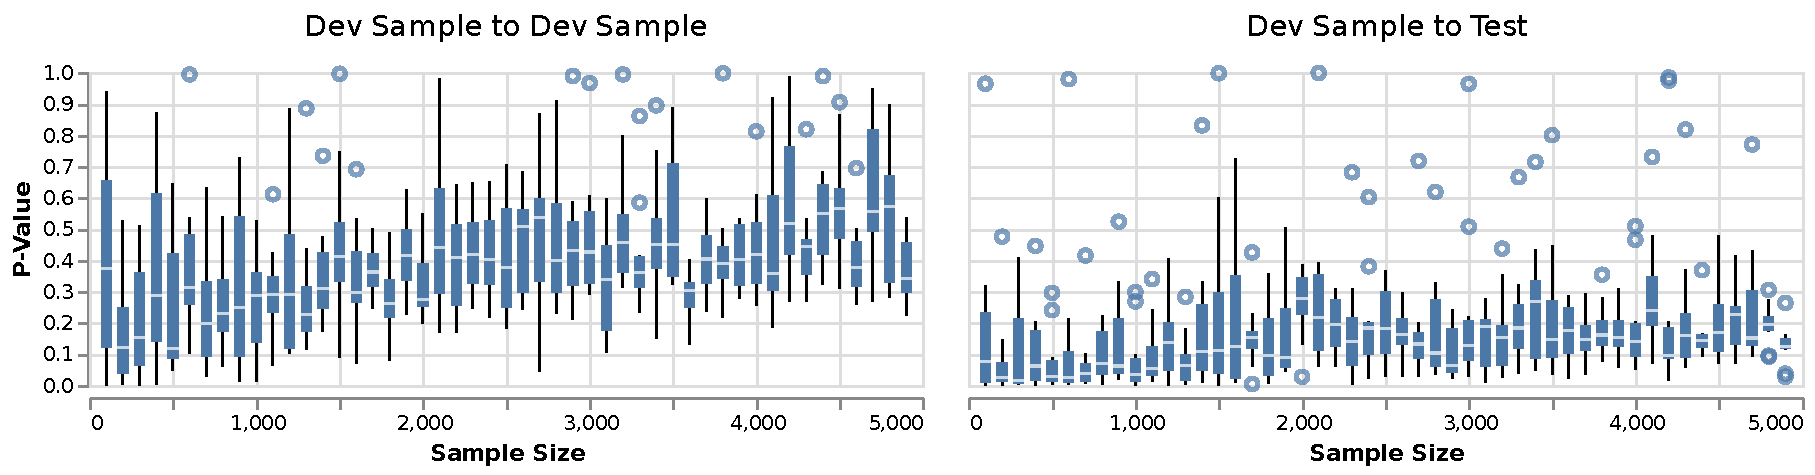
\includegraphics[width=\textwidth]{ranking_stability_significance}
  \caption{
    P-values of the rank correlation difference for each sample size and trial in Figure~\ref{fig:stability}.
    The inherent noise in dev set sampling makes inferring significance difficult (left); test set driven results (right) are more significant.
  }
  \label{fig:rank_sig}
\end{figure*}


\section{The IRT Statistical Test}
\label{ch:isicle:irt-test}

The \irt{} test differs in two substantial ways from other tests: (1) it does not assume that \itms{} are equally informative and (2) it does assume that the informativeness of \itms{} is a function of the \subj{}'s skill $\theta_j$.
In the literature, this is closely connected to \iemph{reliability}~\citep{sutcliffe1992pragmatics} and each \itm{} provides information about the location of $\theta_j$; as we accumulate more evidence for the location of $\theta_j$ the error of estimation decreases.
It is a well known result in \irt{} that standard error of estimate (\abr{see}) $\sigma(\hat{\theta}|\theta)$ varies with respect to the agent location parameter $\theta$~\citep[p.~30]{theory2013ayala} and is connected to the Fisher information
\begin{equation}
  I_i(\theta)=\frac{(p_i')^2}{p_i(1-p_i)}
\end{equation}
of each item.
For a 2PL model, information
\begin{equation}
  I_i(\theta)=\gamma^2p_i(1-p_i)
\end{equation}
is maximized when $p_i=(1-p_i)$.
Since Fisher information is additive, the information of the evaluation set is maximal when \itms{} have a $50\%$ chance of being responded to correctly.
As derived by~\citet[p.~102]{theory2013ayala}, the standard error of estimation
\begin{equation}
  \text{SEE}(\theta)=\sqrt{\frac{1}{\sum_i I_i(\theta)}}.
\end{equation}
is computed by accumulating the information gained from each \itm{}.
Given two \subjs{} $X$ and $Y$, one can use the probability distribution of score differences
\begin{equation}
  N(\theta_Y-\theta_X, \text{SEE}(\theta_X)^2+\text{SEE}(\theta_Y)^2)
\end{equation}
to compute the probability that the difference in skill is greater than two standard errors which corresponds to an $\alpha\le .05$ significance level.
%derive error apx~\citep{hambleton1991fundamentals}

\section{Multidimensional IRT Clustering}
\label{ch:isicle:clustering}

While we achieve strong held-out accuracy with 10 dimensional \irt{} (\pl{m}), we had limited success in interpreting parameters.
We use \abr{tsne}\footnote{
  We use openTSNE~\citep{policar2019tsne} with default parameters.
} plots overlayed with features like \itm{} accuracy, the question's Wikipedia page, if the question was answerable, length of questions, and topic model weights.
Of these, \itm{} accuracy and answerability showed the most obvious patterns (Figure~\ref{fig:tsne-squad}).

\begin{figure}[t]
  \centering
  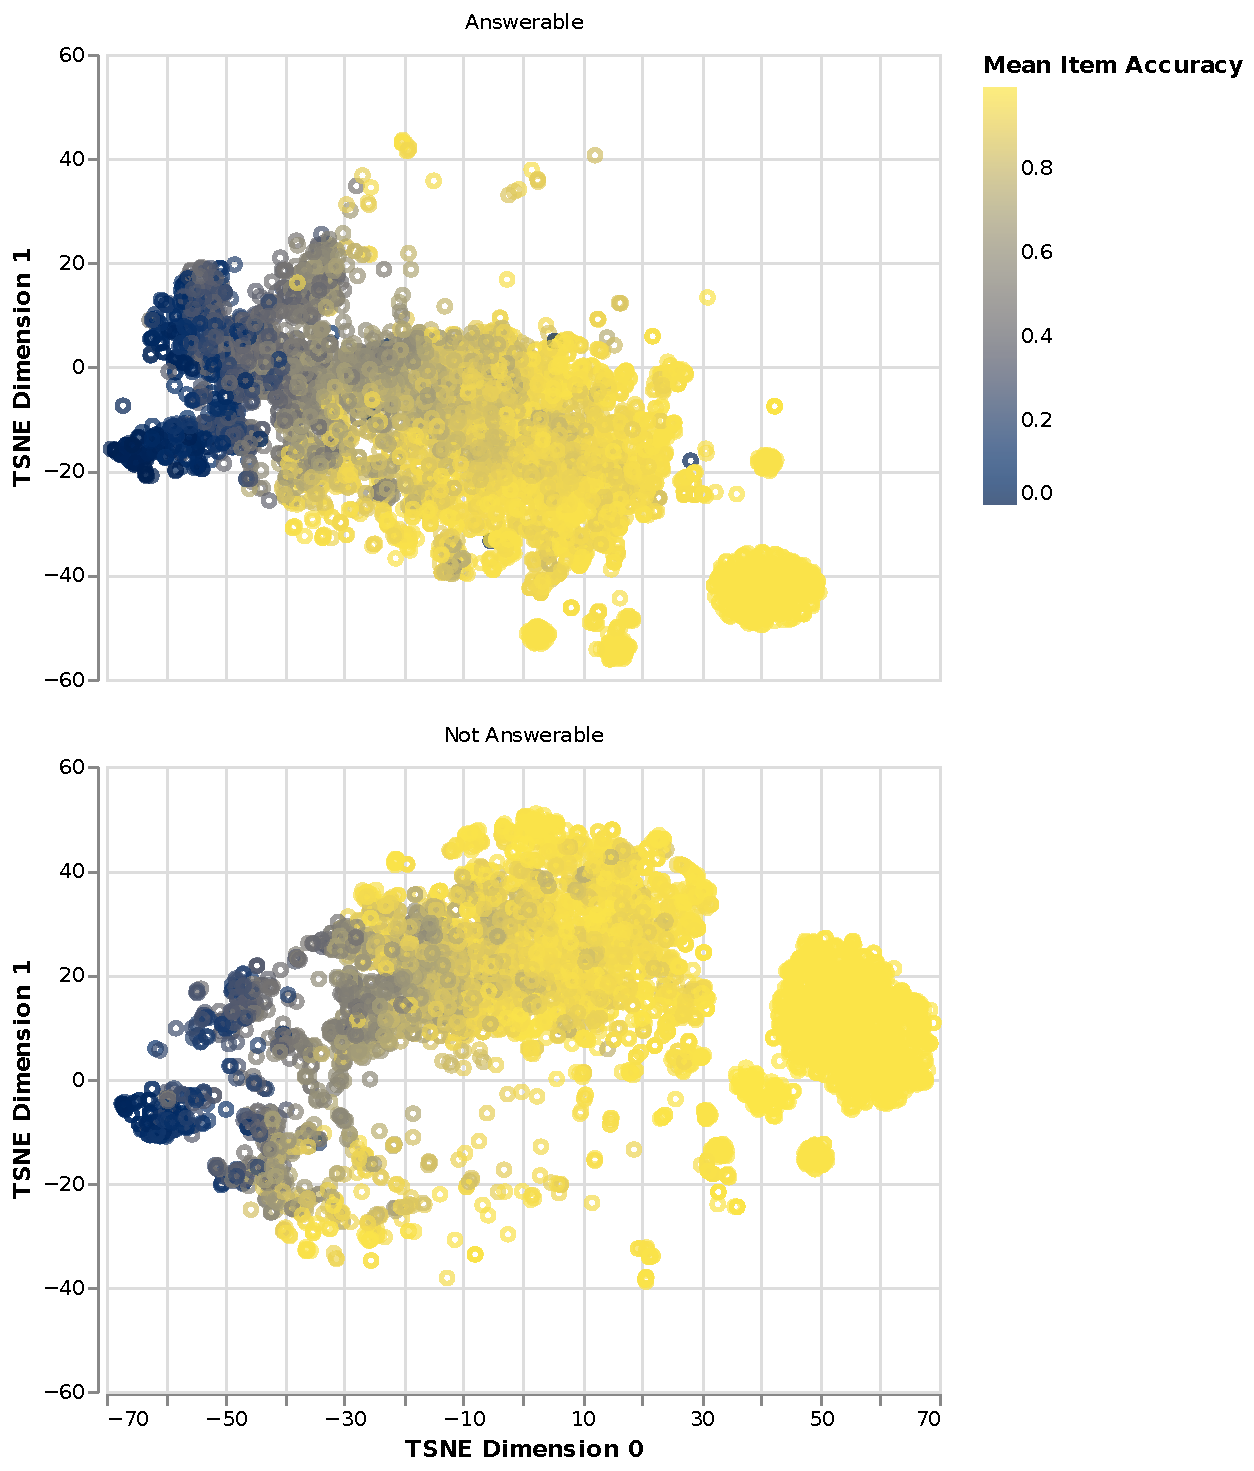
\includegraphics[width=\columnwidth]{squad_tsne}
  \caption{
    In \squad{}, \abr{tsne} shows a relationship between mean exact match (\itm{} accuracy) and answerability with respect to multidimensional \diff{} and \discability{}.
  }
  \label{fig:tsne-squad}
\end{figure}

We repeated this approach with the multi-task question answering shared task \abr{mrqa}~\citep{fisch2019mrqa}.
However, instead of using 10 dimensions we use 6 to match the number of development set tasks in \abr{mrqa}.
Although questions in NarrativeQA standout (Figure~\ref{fig:tsne-mrqa}), there is not a discernible pattern amongst the other tasks.
We leave more sophisticated methods for making multidimensional \irt{} models interpretable to future work.

\begin{figure}[t]
  \centering
  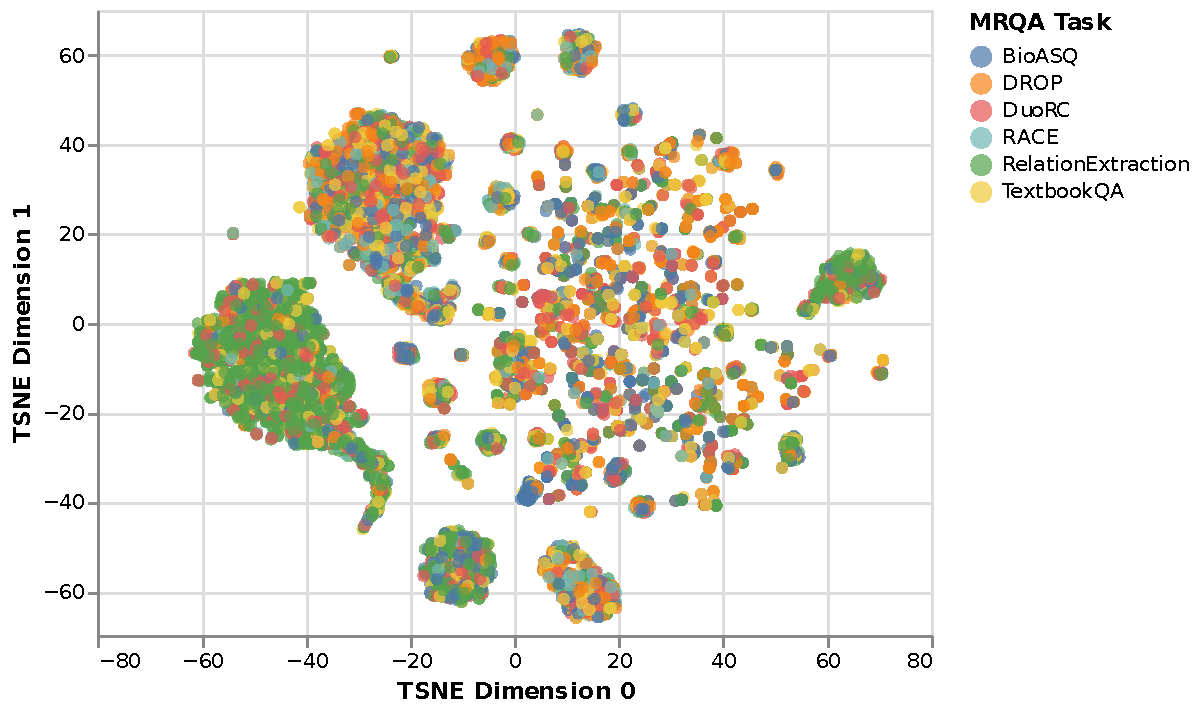
\includegraphics[width=\columnwidth]{mrqa_tsne}
  \caption{
    In \abr{mrqa}, \abr{tsne} shows a relationship between whether the task is NarrativeQA with respect to multidimensional \diff{} and \discability{}.
  }
  \label{fig:tsne-mrqa}
\end{figure}



\section{Reproducibility Checklist}

Here we provide reproducibility details to complement our source code (\href{https://irt.pedro.ai}{https://irt.pedro.ai}).

\subsection{Software and Parameters}

All \irt{} models are implemented in PyTorch~\citep{pytorch2019} and Pyro~\citep{bingham2018pyro}.
Linear models are trained with Vowpal Wabbit~\citep{Agarwal2014ARE}.
The topic model that generates features for the linear model uses Mallet~\citep{McCallumMALLET}.

The number of \irt{} model parameters is proportional to the number of \subjs{} $m$ and the number of \itms{} $n$.
The \pl{1}~has one parameter per \subj{} and one per \itm{}.
The \pl{2}~has one parameter per \subj{} and two per \itm{}.
The \pl{3}~has one parameter per \subj{} and three per \itm{}.
The \pl{m}~has ten parameters per \subj{} and thirty per \itm{}.

\subsection{Hyperparameters}

We did not invest significant effort in hyper-parameter tuning the \irt{} models and instead used the defaults in the py-irt software\footnote{\href{https://github.com/jplalor/py-irt}{github.com/jplalor/py-irt}} provided by~\citet{lalor2019latent}.
The \pl{1}, \pl{2}, and \pl{3}~models were trained for 1000 epochs with no early stopping conditions and a learning rate of $0.1$ with \abr{adam}~\citep{Kingma2014AdamAM}.
The \pl{m}~model was trained for 2500 epochs and used 10 dimensions.

In the linear model, we used a Hyperopt-based~\citep{bergstra2013hyperopt} tool provided by Vowpal Wabbit\footnote{
  \href{https://github.com/VowpalWabbit/vowpal_wabbit}{github.com/VowpalWabbit/vowpal\_wabbit}
} for hyper parameter search.
For each \abr{lm}, the tool spent 20 iterations optimizing the learning rate, L2 regularization, and number of bits against the logistic loss function.
The learning rate was searched from 0.001 to 10 with loguniform sampling, L2 regularization from $1e-8$ to 1, and bits from 20 to 23 as categorical variables.

The topic model that generated features for the linear model used mallet, and we followed the recommendations of the software to set hyper parameters.\footnote{
  \href{http://mallet.cs.umass.edu/topics.php}{mallet.cs.umass.edu/topics.php}
}
Specifically, we used an optimization interval of 10, removed stop words, trained for 1000 iterations, and used a document-topic threshold of 0.05.
Each document was comprised of the Wikipedia page title and the question text.

\subsection{Computational Resources}

The majority of experiments were conducted on a single workstation with an Intel i7-7700K \abr{cpu}, $47$\abr{gb} of \abr{ram}, and an Nvidia 1080Ti.
The average runtime for the \pl{3}~model on \abr{cpu} is 113 seconds with a standard deviation of 2.31 over 5 trials.
The average runtime of the \pl{m}~model on \abr{gpu} is 110 seconds with a standard deviation of 0.5 over 5 trials.

Since each ranking stability experiment required (\S\ref{ch:isicle:stable}) re-training an \pl{3}~model on each subset, we parallelized this experiment on a \abr{cpu} cluster where each trial received two \abr{cpu} cores and 16\abr{gb} of \abr{ram}.
In total, this included 520 trials which corresponds to twice that many trained \irt{} models since one model is trained on each subset of the data.
